% Created by tikzDevice version 0.8.1 on 2015-06-28 21:35:40
% !TEX encoding = UTF-8 Unicode
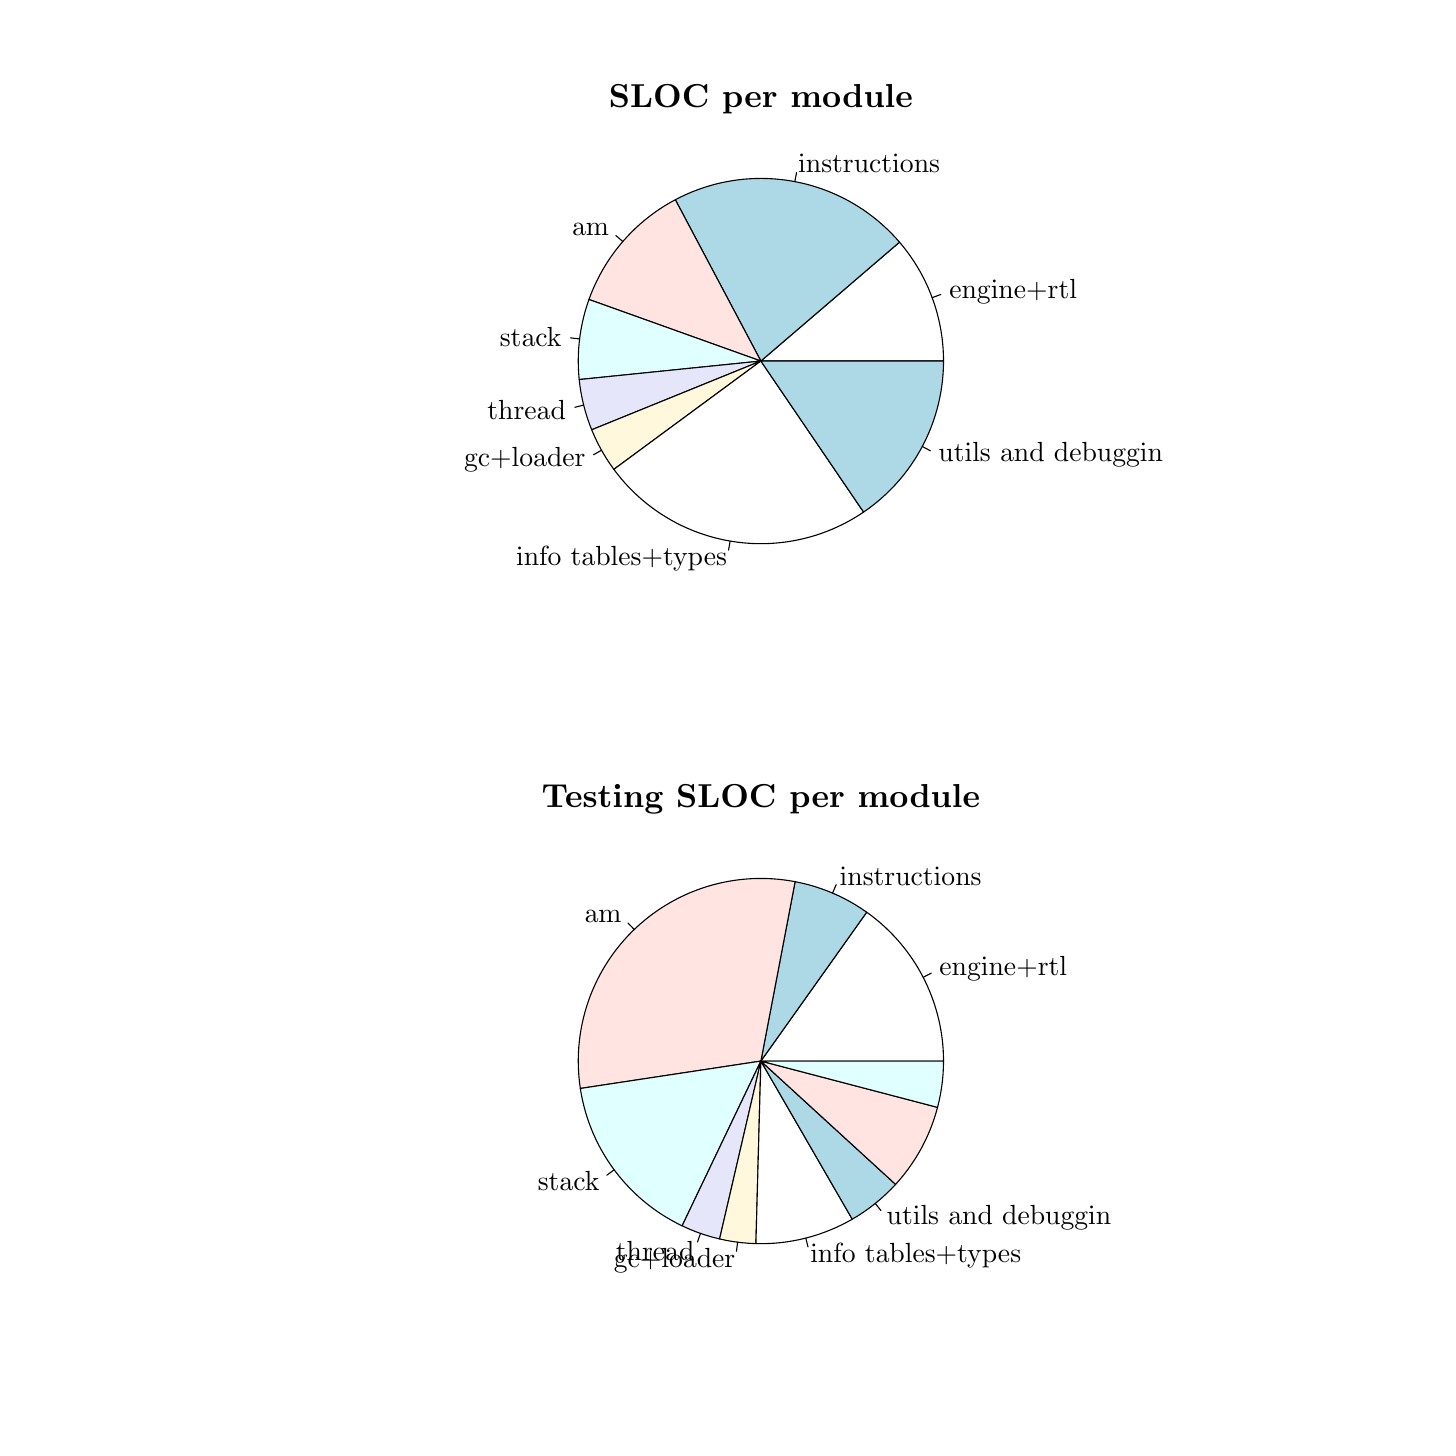
\begin{tikzpicture}[x=1pt,y=1pt]
\definecolor{fillColor}{RGB}{255,255,255}
\path[use as bounding box,fill=fillColor,fill opacity=0.00] (0,0) rectangle (505.89,505.89);
\begin{scope}
\path[clip] ( 49.20,314.14) rectangle (480.69,456.69);
\definecolor{drawColor}{RGB}{0,0,0}
\definecolor{fillColor}{RGB}{255,255,255}

\path[draw=drawColor,line width= 0.4pt,line join=round,line cap=round,fill=fillColor] (330.94,385.42) --
	(330.90,387.64) --
	(330.79,389.87) --
	(330.60,392.09) --
	(330.34,394.30) --
	(330.00,396.50) --
	(329.59,398.69) --
	(329.10,400.87) --
	(328.55,403.02) --
	(327.92,405.16) --
	(327.21,407.27) --
	(326.44,409.36) --
	(325.60,411.43) --
	(324.68,413.46) --
	(323.70,415.46) --
	(322.66,417.42) --
	(321.54,419.35) --
	(320.37,421.24) --
	(319.13,423.09) --
	(317.82,424.90) --
	(316.46,426.66) --
	(315.04,428.38) --
	(264.94,385.42) --
	cycle;

\path[draw=drawColor,line width= 0.4pt,line join=round,line cap=round] (326.84,408.32) --
	(329.93,409.47);
\end{scope}
\begin{scope}
\path[clip] (  0.00,252.94) rectangle (505.89,505.89);
\definecolor{drawColor}{RGB}{0,0,0}

\node[text=drawColor,anchor=base west,inner sep=0pt, outer sep=0pt, scale=  1.00] at (333.02,408.14) {engine+rtl};
\end{scope}
\begin{scope}
\path[clip] ( 49.20,314.14) rectangle (480.69,456.69);
\definecolor{drawColor}{RGB}{0,0,0}
\definecolor{fillColor}{RGB}{173,216,230}

\path[draw=drawColor,line width= 0.4pt,line join=round,line cap=round,fill=fillColor] (315.04,428.38) --
	(313.60,430.00) --
	(312.10,431.58) --
	(310.56,433.11) --
	(308.96,434.58) --
	(307.32,436.01) --
	(305.63,437.37) --
	(303.90,438.68) --
	(302.13,439.94) --
	(300.31,441.13) --
	(298.46,442.27) --
	(296.57,443.34) --
	(294.65,444.35) --
	(292.69,445.29) --
	(290.71,446.17) --
	(288.69,446.99) --
	(286.65,447.74) --
	(284.59,448.42) --
	(282.51,449.03) --
	(280.40,449.57) --
	(278.28,450.05) --
	(276.15,450.45) --
	(274.00,450.79) --
	(271.85,451.05) --
	(269.68,451.24) --
	(267.51,451.36) --
	(265.34,451.41) --
	(263.17,451.39) --
	(261.00,451.29) --
	(258.83,451.13) --
	(256.67,450.89) --
	(254.52,450.58) --
	(252.38,450.20) --
	(250.26,449.76) --
	(248.15,449.24) --
	(246.06,448.65) --
	(243.99,447.99) --
	(241.94,447.27) --
	(239.91,446.48) --
	(237.92,445.62) --
	(235.95,444.70) --
	(234.02,443.71) --
	(264.94,385.42) --
	cycle;

\path[draw=drawColor,line width= 0.4pt,line join=round,line cap=round] (277.22,450.26) --
	(277.83,453.50);
\end{scope}
\begin{scope}
\path[clip] (  0.00,252.94) rectangle (505.89,505.89);
\definecolor{drawColor}{RGB}{0,0,0}

\node[text=drawColor,anchor=base west,inner sep=0pt, outer sep=0pt, scale=  1.00] at (278.44,453.43) {instructions};
\end{scope}
\begin{scope}
\path[clip] ( 49.20,314.14) rectangle (480.69,456.69);
\definecolor{drawColor}{RGB}{0,0,0}
\definecolor{fillColor}{RGB}{255,228,225}

\path[draw=drawColor,line width= 0.4pt,line join=round,line cap=round,fill=fillColor] (234.02,443.71) --
	(232.08,442.64) --
	(230.17,441.51) --
	(228.31,440.31) --
	(226.49,439.05) --
	(224.71,437.72) --
	(222.97,436.34) --
	(221.28,434.90) --
	(219.65,433.41) --
	(218.06,431.86) --
	(216.53,430.26) --
	(215.05,428.61) --
	(213.63,426.91) --
	(212.26,425.16) --
	(210.96,423.37) --
	(209.71,421.53) --
	(208.53,419.66) --
	(207.41,417.75) --
	(206.36,415.79) --
	(205.37,413.81) --
	(204.45,411.79) --
	(203.60,409.75) --
	(202.82,407.67) --
	(264.94,385.42) --
	cycle;

\path[draw=drawColor,line width= 0.4pt,line join=round,line cap=round] (215.05,428.61) --
	(212.55,430.77);
\end{scope}
\begin{scope}
\path[clip] (  0.00,252.94) rectangle (505.89,505.89);
\definecolor{drawColor}{RGB}{0,0,0}

\node[text=drawColor,anchor=base east,inner sep=0pt, outer sep=0pt, scale=  1.00] at (210.06,430.78) {am};
\end{scope}
\begin{scope}
\path[clip] ( 49.20,314.14) rectangle (480.69,456.69);
\definecolor{drawColor}{RGB}{0,0,0}
\definecolor{fillColor}{RGB}{224,255,255}

\path[draw=drawColor,line width= 0.4pt,line join=round,line cap=round,fill=fillColor] (202.82,407.67) --
	(202.09,405.53) --
	(201.44,403.36) --
	(200.86,401.18) --
	(200.36,398.97) --
	(199.93,396.75) --
	(199.58,394.52) --
	(199.31,392.27) --
	(199.11,390.02) --
	(198.99,387.76) --
	(198.95,385.50) --
	(198.99,383.24) --
	(199.10,380.98) --
	(199.29,378.73) --
	(264.94,385.42) --
	cycle;

\path[draw=drawColor,line width= 0.4pt,line join=round,line cap=round] (199.44,393.40) --
	(196.16,393.80);
\end{scope}
\begin{scope}
\path[clip] (  0.00,252.94) rectangle (505.89,505.89);
\definecolor{drawColor}{RGB}{0,0,0}

\node[text=drawColor,anchor=base east,inner sep=0pt, outer sep=0pt, scale=  1.00] at (192.89,390.75) {stack};
\end{scope}
\begin{scope}
\path[clip] ( 49.20,314.14) rectangle (480.69,456.69);
\definecolor{drawColor}{RGB}{0,0,0}
\definecolor{fillColor}{RGB}{230,230,250}

\path[draw=drawColor,line width= 0.4pt,line join=round,line cap=round,fill=fillColor] (199.29,378.73) --
	(199.57,376.40) --
	(199.93,374.08) --
	(200.38,371.78) --
	(200.90,369.49) --
	(201.51,367.23) --
	(202.20,364.98) --
	(202.96,362.77) --
	(203.81,360.58) --
	(264.94,385.42) --
	cycle;

\path[draw=drawColor,line width= 0.4pt,line join=round,line cap=round] (200.90,369.49) --
	(197.70,368.70);
\end{scope}
\begin{scope}
\path[clip] (  0.00,252.94) rectangle (505.89,505.89);
\definecolor{drawColor}{RGB}{0,0,0}

\node[text=drawColor,anchor=base east,inner sep=0pt, outer sep=0pt, scale=  1.00] at (194.50,364.46) {thread};
\end{scope}
\begin{scope}
\path[clip] ( 49.20,314.14) rectangle (480.69,456.69);
\definecolor{drawColor}{RGB}{0,0,0}
\definecolor{fillColor}{RGB}{255,248,220}

\path[draw=drawColor,line width= 0.4pt,line join=round,line cap=round,fill=fillColor] (203.81,360.58) --
	(204.89,358.06) --
	(206.07,355.60) --
	(207.36,353.18) --
	(208.75,350.82) --
	(210.23,348.52) --
	(211.81,346.28) --
	(264.94,385.42) --
	cycle;

\path[draw=drawColor,line width= 0.4pt,line join=round,line cap=round] (207.36,353.18) --
	(204.48,351.57);
\end{scope}
\begin{scope}
\path[clip] (  0.00,252.94) rectangle (505.89,505.89);
\definecolor{drawColor}{RGB}{0,0,0}

\node[text=drawColor,anchor=base east,inner sep=0pt, outer sep=0pt, scale=  1.00] at (201.60,347.48) {gc+loader};
\end{scope}
\begin{scope}
\path[clip] ( 49.20,314.14) rectangle (480.69,456.69);
\definecolor{drawColor}{RGB}{0,0,0}
\definecolor{fillColor}{RGB}{255,255,255}

\path[draw=drawColor,line width= 0.4pt,line join=round,line cap=round,fill=fillColor] (211.81,346.28) --
	(213.12,344.57) --
	(214.48,342.90) --
	(215.89,341.27) --
	(217.35,339.70) --
	(218.87,338.17) --
	(220.44,336.69) --
	(222.05,335.27) --
	(223.71,333.89) --
	(225.41,332.58) --
	(227.15,331.32) --
	(228.94,330.11) --
	(230.76,328.97) --
	(232.62,327.88) --
	(234.51,326.86) --
	(236.44,325.90) --
	(238.40,325.00) --
	(240.38,324.17) --
	(242.39,323.40) --
	(244.43,322.70) --
	(246.48,322.06) --
	(248.56,321.49) --
	(250.65,320.99) --
	(252.76,320.56) --
	(254.88,320.20) --
	(257.02,319.90) --
	(259.16,319.68) --
	(261.30,319.52) --
	(263.46,319.44) --
	(265.61,319.43) --
	(267.76,319.48) --
	(269.91,319.61) --
	(272.05,319.81) --
	(274.19,320.07) --
	(276.31,320.41) --
	(278.43,320.82) --
	(280.53,321.29) --
	(282.61,321.83) --
	(284.68,322.44) --
	(286.72,323.12) --
	(288.74,323.86) --
	(290.73,324.67) --
	(292.70,325.55) --
	(294.64,326.48) --
	(296.55,327.48) --
	(298.42,328.54) --
	(300.26,329.67) --
	(302.05,330.85) --
	(264.94,385.42) --
	cycle;

\path[draw=drawColor,line width= 0.4pt,line join=round,line cap=round] (253.82,320.37) --
	(253.27,317.12);
\end{scope}
\begin{scope}
\path[clip] (  0.00,252.94) rectangle (505.89,505.89);
\definecolor{drawColor}{RGB}{0,0,0}

\node[text=drawColor,anchor=base east,inner sep=0pt, outer sep=0pt, scale=  1.00] at (252.71,311.39) {info tables+types};
\end{scope}
\begin{scope}
\path[clip] ( 49.20,314.14) rectangle (480.69,456.69);
\definecolor{drawColor}{RGB}{0,0,0}
\definecolor{fillColor}{RGB}{173,216,230}

\path[draw=drawColor,line width= 0.4pt,line join=round,line cap=round,fill=fillColor] (302.05,330.85) --
	(303.87,332.12) --
	(305.63,333.46) --
	(307.35,334.85) --
	(309.03,336.31) --
	(310.65,337.81) --
	(312.22,339.37) --
	(313.74,340.99) --
	(315.21,342.65) --
	(316.61,344.36) --
	(317.96,346.12) --
	(319.25,347.92) --
	(320.48,349.76) --
	(321.64,351.65) --
	(322.75,353.57) --
	(323.78,355.53) --
	(324.75,357.52) --
	(325.65,359.54) --
	(326.49,361.60) --
	(327.25,363.68) --
	(327.95,365.78) --
	(328.57,367.91) --
	(329.12,370.05) --
	(329.60,372.21) --
	(330.01,374.39) --
	(330.34,376.58) --
	(330.60,378.78) --
	(330.79,380.99) --
	(330.90,383.20) --
	(330.94,385.42) --
	(264.94,385.42) --
	cycle;

\path[draw=drawColor,line width= 0.4pt,line join=round,line cap=round] (323.27,354.55) --
	(326.19,353.00);
\end{scope}
\begin{scope}
\path[clip] (  0.00,252.94) rectangle (505.89,505.89);
\definecolor{drawColor}{RGB}{0,0,0}

\node[text=drawColor,anchor=base west,inner sep=0pt, outer sep=0pt, scale=  1.00] at (329.10,348.99) {utils and debuggin};

\node[text=drawColor,anchor=base,inner sep=0pt, outer sep=0pt, scale=  1.20] at (264.94,477.15) {\bfseries SLOC per module};
\end{scope}
\begin{scope}
\path[clip] ( 49.20, 61.20) rectangle (480.69,203.75);
\definecolor{drawColor}{RGB}{0,0,0}
\definecolor{fillColor}{RGB}{255,255,255}

\path[draw=drawColor,line width= 0.4pt,line join=round,line cap=round,fill=fillColor] (330.94,132.47) --
	(330.90,134.64) --
	(330.80,136.81) --
	(330.62,138.97) --
	(330.37,141.12) --
	(330.05,143.27) --
	(329.66,145.40) --
	(329.20,147.52) --
	(328.67,149.62) --
	(328.07,151.70) --
	(327.41,153.77) --
	(326.67,155.81) --
	(325.87,157.82) --
	(325.01,159.81) --
	(324.08,161.77) --
	(323.08,163.70) --
	(322.03,165.59) --
	(320.91,167.45) --
	(319.73,169.27) --
	(318.49,171.05) --
	(317.19,172.78) --
	(315.84,174.48) --
	(314.44,176.13) --
	(312.97,177.73) --
	(311.46,179.28) --
	(309.90,180.79) --
	(308.29,182.24) --
	(306.63,183.63) --
	(304.93,184.98) --
	(303.18,186.26) --
	(264.94,132.47) --
	cycle;

\path[draw=drawColor,line width= 0.4pt,line join=round,line cap=round] (323.59,162.74) --
	(326.52,164.25);
\end{scope}
\begin{scope}
\path[clip] (  0.00,  0.00) rectangle (505.89,252.94);
\definecolor{drawColor}{RGB}{0,0,0}

\node[text=drawColor,anchor=base west,inner sep=0pt, outer sep=0pt, scale=  1.00] at (329.45,163.29) {engine+rtl};
\end{scope}
\begin{scope}
\path[clip] ( 49.20, 61.20) rectangle (480.69,203.75);
\definecolor{drawColor}{RGB}{0,0,0}
\definecolor{fillColor}{RGB}{173,216,230}

\path[draw=drawColor,line width= 0.4pt,line join=round,line cap=round,fill=fillColor] (303.18,186.26) --
	(301.23,187.59) --
	(299.24,188.86) --
	(297.20,190.05) --
	(295.12,191.17) --
	(293.00,192.21) --
	(290.84,193.17) --
	(288.65,194.06) --
	(286.43,194.87) --
	(284.19,195.60) --
	(281.92,196.25) --
	(279.62,196.81) --
	(277.31,197.30) --
	(264.94,132.47) --
	cycle;

\path[draw=drawColor,line width= 0.4pt,line join=round,line cap=round] (290.84,193.17) --
	(292.14,196.21);
\end{scope}
\begin{scope}
\path[clip] (  0.00,  0.00) rectangle (505.89,252.94);
\definecolor{drawColor}{RGB}{0,0,0}

\node[text=drawColor,anchor=base west,inner sep=0pt, outer sep=0pt, scale=  1.00] at (293.43,195.93) {instructions};
\end{scope}
\begin{scope}
\path[clip] ( 49.20, 61.20) rectangle (480.69,203.75);
\definecolor{drawColor}{RGB}{0,0,0}
\definecolor{fillColor}{RGB}{255,228,225}

\path[draw=drawColor,line width= 0.4pt,line join=round,line cap=round,fill=fillColor] (277.31,197.30) --
	(275.21,197.66) --
	(273.09,197.96) --
	(270.97,198.19) --
	(268.84,198.35) --
	(266.71,198.44) --
	(264.57,198.46) --
	(262.43,198.42) --
	(260.30,198.30) --
	(258.17,198.12) --
	(256.05,197.86) --
	(253.94,197.54) --
	(251.84,197.15) --
	(249.75,196.69) --
	(247.68,196.17) --
	(245.63,195.58) --
	(243.60,194.92) --
	(241.59,194.19) --
	(239.60,193.41) --
	(237.64,192.55) --
	(235.71,191.64) --
	(233.81,190.66) --
	(231.95,189.62) --
	(230.11,188.52) --
	(228.32,187.37) --
	(226.56,186.15) --
	(224.84,184.88) --
	(223.17,183.56) --
	(221.54,182.18) --
	(219.95,180.75) --
	(218.41,179.27) --
	(216.92,177.74) --
	(215.48,176.16) --
	(214.09,174.53) --
	(212.76,172.87) --
	(211.48,171.16) --
	(210.25,169.40) --
	(209.09,167.61) --
	(207.98,165.79) --
	(206.93,163.93) --
	(205.94,162.03) --
	(205.02,160.11) --
	(204.15,158.15) --
	(203.35,156.17) --
	(202.62,154.17) --
	(201.95,152.14) --
	(201.35,150.09) --
	(200.81,148.02) --
	(200.34,145.94) --
	(199.94,143.84) --
	(199.60,141.73) --
	(199.34,139.61) --
	(199.14,137.48) --
	(199.01,135.35) --
	(198.96,133.21) --
	(198.97,131.08) --
	(199.05,128.94) --
	(199.20,126.81) --
	(199.41,124.69) --
	(199.70,122.57) --
	(264.94,132.47) --
	cycle;

\path[draw=drawColor,line width= 0.4pt,line join=round,line cap=round] (219.17,180.01) --
	(216.89,182.39);
\end{scope}
\begin{scope}
\path[clip] (  0.00,  0.00) rectangle (505.89,252.94);
\definecolor{drawColor}{RGB}{0,0,0}

\node[text=drawColor,anchor=base east,inner sep=0pt, outer sep=0pt, scale=  1.00] at (214.60,182.61) {am};
\end{scope}
\begin{scope}
\path[clip] ( 49.20, 61.20) rectangle (480.69,203.75);
\definecolor{drawColor}{RGB}{0,0,0}
\definecolor{fillColor}{RGB}{224,255,255}

\path[draw=drawColor,line width= 0.4pt,line join=round,line cap=round,fill=fillColor] (199.70,122.57) --
	(200.05,120.46) --
	(200.48,118.36) --
	(200.97,116.27) --
	(201.53,114.20) --
	(202.16,112.15) --
	(202.85,110.13) --
	(203.61,108.12) --
	(204.43,106.14) --
	(205.32,104.19) --
	(206.27,102.27) --
	(207.28,100.38) --
	(208.35, 98.53) --
	(209.48, 96.71) --
	(210.67, 94.92) --
	(211.92, 93.18) --
	(213.23, 91.48) --
	(214.58, 89.82) --
	(216.00, 88.21) --
	(217.46, 86.65) --
	(218.97, 85.13) --
	(220.53, 83.66) --
	(222.14, 82.24) --
	(223.79, 80.88) --
	(225.49, 79.57) --
	(227.23, 78.32) --
	(229.01, 77.12) --
	(230.82, 75.99) --
	(232.68, 74.91) --
	(234.56, 73.89) --
	(236.48, 72.93) --
	(264.94,132.47) --
	cycle;

\path[draw=drawColor,line width= 0.4pt,line join=round,line cap=round] (211.92, 93.18) --
	(209.27, 91.22);
\end{scope}
\begin{scope}
\path[clip] (  0.00,  0.00) rectangle (505.89,252.94);
\definecolor{drawColor}{RGB}{0,0,0}

\node[text=drawColor,anchor=base east,inner sep=0pt, outer sep=0pt, scale=  1.00] at (206.62, 85.81) {stack};
\end{scope}
\begin{scope}
\path[clip] ( 49.20, 61.20) rectangle (480.69,203.75);
\definecolor{drawColor}{RGB}{0,0,0}
\definecolor{fillColor}{RGB}{230,230,250}

\path[draw=drawColor,line width= 0.4pt,line join=round,line cap=round,fill=fillColor] (236.48, 72.93) --
	(239.10, 71.75) --
	(241.77, 70.68) --
	(244.48, 69.73) --
	(247.24, 68.90) --
	(250.02, 68.19) --
	(264.94,132.47) --
	cycle;

\path[draw=drawColor,line width= 0.4pt,line join=round,line cap=round] (243.12, 70.19) --
	(242.03, 67.08);
\end{scope}
\begin{scope}
\path[clip] (  0.00,  0.00) rectangle (505.89,252.94);
\definecolor{drawColor}{RGB}{0,0,0}

\node[text=drawColor,anchor=base east,inner sep=0pt, outer sep=0pt, scale=  1.00] at (240.94, 60.52) {thread};
\end{scope}
\begin{scope}
\path[clip] ( 49.20, 61.20) rectangle (480.69,203.75);
\definecolor{drawColor}{RGB}{0,0,0}
\definecolor{fillColor}{RGB}{255,248,220}

\path[draw=drawColor,line width= 0.4pt,line join=round,line cap=round,fill=fillColor] (250.02, 68.19) --
	(252.62, 67.64) --
	(255.23, 67.20) --
	(257.86, 66.86) --
	(260.50, 66.63) --
	(263.15, 66.50) --
	(264.94,132.47) --
	cycle;

\path[draw=drawColor,line width= 0.4pt,line join=round,line cap=round] (256.54, 67.02) --
	(256.12, 63.74);
\end{scope}
\begin{scope}
\path[clip] (  0.00,  0.00) rectangle (505.89,252.94);
\definecolor{drawColor}{RGB}{0,0,0}

\node[text=drawColor,anchor=base east,inner sep=0pt, outer sep=0pt, scale=  1.00] at (255.70, 58.00) {gc+loader};
\end{scope}
\begin{scope}
\path[clip] ( 49.20, 61.20) rectangle (480.69,203.75);
\definecolor{drawColor}{RGB}{0,0,0}
\definecolor{fillColor}{RGB}{255,255,255}

\path[draw=drawColor,line width= 0.4pt,line join=round,line cap=round,fill=fillColor] (263.15, 66.50) --
	(265.42, 66.48) --
	(267.69, 66.54) --
	(269.96, 66.67) --
	(272.23, 66.88) --
	(274.48, 67.17) --
	(276.72, 67.54) --
	(278.95, 67.98) --
	(281.17, 68.50) --
	(283.36, 69.10) --
	(285.53, 69.77) --
	(287.68, 70.52) --
	(289.80, 71.34) --
	(291.89, 72.23) --
	(293.95, 73.20) --
	(295.97, 74.23) --
	(297.96, 75.33) --
	(264.94,132.47) --
	cycle;

\path[draw=drawColor,line width= 0.4pt,line join=round,line cap=round] (281.17, 68.50) --
	(281.98, 65.31);
\end{scope}
\begin{scope}
\path[clip] (  0.00,  0.00) rectangle (505.89,252.94);
\definecolor{drawColor}{RGB}{0,0,0}

\node[text=drawColor,anchor=base west,inner sep=0pt, outer sep=0pt, scale=  1.00] at (282.79, 59.64) {info tables+types};
\end{scope}
\begin{scope}
\path[clip] ( 49.20, 61.20) rectangle (480.69,203.75);
\definecolor{drawColor}{RGB}{0,0,0}
\definecolor{fillColor}{RGB}{173,216,230}

\path[draw=drawColor,line width= 0.4pt,line join=round,line cap=round,fill=fillColor] (297.96, 75.33) --
	(300.12, 76.63) --
	(302.23, 78.02) --
	(304.28, 79.48) --
	(306.27, 81.02) --
	(308.21, 82.64) --
	(310.08, 84.33) --
	(311.88, 86.08) --
	(313.62, 87.91) --
	(264.94,132.47) --
	cycle;

\path[draw=drawColor,line width= 0.4pt,line join=round,line cap=round] (306.27, 81.02) --
	(308.34, 78.45);
\end{scope}
\begin{scope}
\path[clip] (  0.00,  0.00) rectangle (505.89,252.94);
\definecolor{drawColor}{RGB}{0,0,0}

\node[text=drawColor,anchor=base west,inner sep=0pt, outer sep=0pt, scale=  1.00] at (310.40, 73.41) {utils and debuggin};
\end{scope}
\begin{scope}
\path[clip] ( 49.20, 61.20) rectangle (480.69,203.75);
\definecolor{drawColor}{RGB}{0,0,0}
\definecolor{fillColor}{RGB}{255,228,225}

\path[draw=drawColor,line width= 0.4pt,line join=round,line cap=round,fill=fillColor] (313.62, 87.91) --
	(315.13, 89.62) --
	(316.59, 91.39) --
	(317.98, 93.20) --
	(319.31, 95.06) --
	(320.57, 96.96) --
	(321.77, 98.91) --
	(322.90,100.90) --
	(323.95,102.93) --
	(324.94,104.99) --
	(325.86,107.08) --
	(326.70,109.21) --
	(327.47,111.36) --
	(328.16,113.54) --
	(328.78,115.74) --
	(264.94,132.47) --
	cycle;
\definecolor{fillColor}{RGB}{224,255,255}

\path[draw=drawColor,line width= 0.4pt,line join=round,line cap=round,fill=fillColor] (328.78,115.74) --
	(329.35,118.09) --
	(329.83,120.46) --
	(330.23,122.84) --
	(330.54,125.24) --
	(330.76,127.64) --
	(330.89,130.06) --
	(330.94,132.47) --
	(264.94,132.47) --
	cycle;
\end{scope}
\begin{scope}
\path[clip] (  0.00,  0.00) rectangle (505.89,252.94);
\definecolor{drawColor}{RGB}{0,0,0}

\node[text=drawColor,anchor=base,inner sep=0pt, outer sep=0pt, scale=  1.20] at (264.94,224.20) {\bfseries Testing SLOC per module};
\end{scope}
\end{tikzpicture}
